\documentclass[11pt]{amsart}
\usepackage[demo]{graphicx}
\usepackage{subfigure}
\usepackage{parcolumns}

\usepackage[dutch]{babel}
\usepackage{a4wide}
%\setlength{\parindent}{0pt}

\newtheorem*{vraag}{Vraag}
\newtheorem*{uitwerking}{Uitwerking}
\newtheorem*{algoritme}{Algoritme}

\newcommand{\R}{\mathbb{R}}
\newcommand{\N}{\mathbb{N}}
\newcommand{\Z}{\mathbb{Z}}
\newcommand{\C}{\mathbb{C}}
\newcommand{\A}{\mathbb{A}}
\newcommand{\Q}{\mathbb{Q}}
\newcommand{\F}{\mathbb{F}}
\newcommand{\f}{\varphi}
\newcommand{\e}{\varepsilon}
\renewcommand{\d}{\delta}

\begin{document}

\section{Intro}
De Fouriertransformatie bestaat al honderden jaren en is een grote speler geworden in de \emph{signal processing}. Een groot nadeel van deze transformatie is dat zij slecht reageert op discontinue signalen.

In de loop van de vorige eeuw is een nieuwe transformatie ontstaan met een eigenschap die de Fouriertransformatie nooit kende. Deze noemt men nu ook wel de Wavelettransformatie.

Een wavelet is simpelweg een functie die voldoet aan
\[
  \int_{-\infty}^{\infty} \psi(t) dt = 0.
\]
Met deze functie $\psi$ kunnen we een familie functies $\psi_{u,s}$ bouwen door middel van schaling en translatie:
\[
  \psi_{u,s}(t) := \frac{1}{\sqrt{s}} \psi\left(\frac{t-u}{s}\right).
\]

Deze familie geeft aanleiding tot een Wavelettransformatie $W_f$ van $f$:
\[
  W_f(u,s) = \int_{-\infty}^\infty f(t) \psi^*_{u,s}(t) dt.
\]

Het is nu mogelijk om wavelets te construeren die met deze schaling en translatie een basis voor de $L_2$ vormen. Over het algemeen kijken we dan naar
\[
  \Psi := \left\{ \psi_{j,n}(t) = \frac{1}{\sqrt{2^j}} \psi\left( \frac{t - 2^jn}{2^j}\right) : (j,n) \in \Z^2 \right\}.
\]
De kunst is nu om de basiselementen loodrecht op elkaar te laten staan, zodat er een orthogonale (en dus een orthonormale) basis gevormd wordt. 

Figuurtje van voorbeeld TODODOO.

Het gevolg is nu dat we elke voldoend nette\footnote{Deze functie moet wel in $L_2$ zitten natuurlijk.} functie kunnen schrijven in deze basis:
\[
  f(t) = \sum_{j=-\infty}^{\infty} \sum_{n=-\infty}^{\infty} \langle f, \psi_{j,n} \rangle \psi_{j,n}(t),
\]
waarbij $\langle \cdot, \cdot \rangle$ het standaardinproduct op de $L_2$ aangeeft.

Het grote nadeel van de Fouriertransformatie maakt compressie van discrete signalen moeilijk. Veel van deze wavelets worden nu z\'o geconstrueerd dat dit probleem (deels) verholpen wordt. We zijn namelijk op zoek naar een wavelet die een eindige drager heeft. Het blijkt dat deze bestaat en dat er zelfs een hele grote verzameling wavelets is, elk met eigen gewilde eigenschappen.

Omdat wij naar de toepassing van wavelets binnen de beeldcompressie bekijken, zijn we natuurlijk vooral ge\"interesseerd in het discrete geval. We kijken dus naar de benadering van $f$ op een TODO. Dit geeft aanleiding tot een rij geneste ruimtes die uiteindelijk naar de $L_2$ toe gaat
\begin{equation}
  \label{multires}
  \{0\} \ldots \subset V_0 \subset V_1 \subset \ldots \subset L_2
\end{equation}
genaamd een multiresolutie.
\subsection{Multiresolutie}
Een rij geneste ruimtes $\{ V_j: j \in \Z \}$ zoals in \eqref{multires} heet een multiresolutie wanneer voldaan wordt aan de volgende eigenschappen:
\[
\begin{array}{c}
  \forall j, k: f(t) \in V_j \implies f(t - 2^j k) \in V_j; \\
  \forall j: V_{j+1} \subset V_j; \\
  \forall j: f(t) \in V_j \iff f(t/2) \in V_{j+1}; \\
  \cap_{j=-\infty}^{\infty} V_{j} = \{0\}; \\
  \cup_{j=-\infty}^{\infty} V_j = L_2. \\
  TODO: \text{ Er is $\phi$ zo dat $\{ \phi(t-n): n \in \Z \}$ een Rieszbasis voor $V_0$ is.}
\end{array}
\]

Als voorbeeld bekijken we een multiresolutie van stuksgewijs constante functies. De ruimte $V_j$ wordt hiermee de verzameling van alle $g(t) \in L_2$ die constant zijn voor $t \in [n 2^j, (n+1)2^j)$ met $n \in \Z$. De basisfunctie $\phi$ voor $V_0$ wordt in dit geval $\phi(t) = 1_{[0,1]}$.

\section{Schalingsfuncties}
Gegeven zo'n Rieszbasis voor $V_0$ willen we graag een orthonormale basis voor $V_j$ construeren. 
TODO: gaan we dit bewijzen? -> stelling 7.1 Mallat
Deze $\theta$ geeft een $\phi$ volgens Mallat. Wanneer we nu defini\"eren
\[
  \phi_{j,n}(t) := \frac{1}{\sqrt{2^j}} \phi\left( \frac{t-n}{2^j} \right),
\]
is $\{ \phi_{j,n}: n \in \Z \}$ een orthonormale basis voor $V_j$.

\subsection{Benadering} TODO.

Met de multiresolutie uit het eerdere voorbeeld kunnen we vinden dat $\{\theta(t-n): n \in \Z \}$ al een orthonormale basis is voor $V_0$, met als gevolg dat $\phi = \theta$.

\section{Filters}
TODO intro.

Per definitie van de multiresolutie weten we dat $V_j \subset V_{j-1}$. In het bijzonder geldt dat $2^{-1/2}\phi(t/2) \in V_1 \subset V_0$ en omdat $\{ \phi(t-n): n \in \Z\}$ een orthonormale basis voor $V_0$ is, kunnen we $2^{-1/2} \phi(t/2)$ nu schrijven als
\[
  \frac{1}{\sqrt{2}} \phi\left(\frac{t}{2}\right) = \sum_{n=-\infty}^{\infty} \left\langle \frac{1}{\sqrt{2}} \phi\left(\frac{t}{2}\right), \phi(t-n) \right\rangle \phi(t-n).
\]
Deze inproducten hebben een speciale naam, want de rij $\{h[n]: n \in \Z\}$ met
\[
  h[n] := \left\langle \frac{1}{\sqrt{2}} \phi\left(\frac{t}{2}\right), \phi(t-n) \right\rangle
\]
wordt nu ook wel de \emph{filter} van $\phi$ genoemd. Andersom, gegeven een $h[n]$ die voldoet aan een aantal voorwaarden, is er een schalingsfunctie $\phi \in L^2(\R)$ waarvoor $h[n]$ de filter is. THEOREM 7.2 TODO?

Om weer terug te komen bij het doorlopende voorbeeld $\phi(t) = 1_{[0,1]}$, vinden we in dit geval dat
\[
  h[n] = \left\langle \frac{1}{\sqrt{2}} \phi\left(\frac{t}{2}\right), \phi(t-n) \right\rangle = \begin{cases} \frac{1}{\sqrt{2}} & \text{ als } n \in \{0,1\} \\ 0 & \text{ anders.} \end{cases}
\]

\section{Eindelijk: wavelets}

\iffalse
\section{Intro}
Het grote nadeel van de Fouriertransformatie is dat een enkele discontinu\"iteit grote gevolgen heeft voor de mate van afname van de co\"effici\"enten. Dit betekent dat compressie in deze gevallen moeilijk wordt. De Waveletbasis is wat anders: elke basisfunctie heeft een compacte drager. Zie de figuur.
\begin{figure}[h]
\subfigure[Impressie van een aantal Fourierbasiselementen]{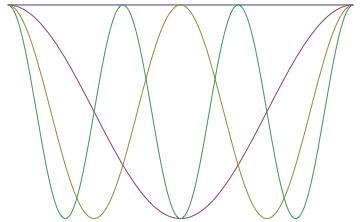
\includegraphics[width=.4\linewidth]{Fourier_basis.jpg}}
\subfigure[Een aantal Morlet-Wavelet basiselementen]{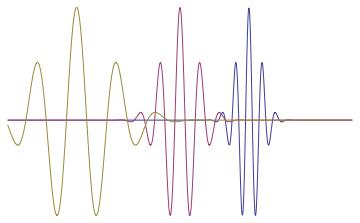
\includegraphics[width=.4\linewidth]{Wavelet_basis.jpg}}
\end{figure}

Het gevolg is dat bij Wavelets een discontinu\"iteit in slechts een deel van de basisfuncties `zichtbaar' zijn. De co\"effici\"enten van de andere basisfuncties nemen op deze manier nog steeds netjes af.

Vanaf nu zullen we (voor het continue geval) aannemen dat een functie/signaal in $L_2$ leeft. Dit is een Hilbertruimte. Laat $\Psi$ een orthonormale basis voor deze ruimte. Als nu een functie $f$ in deze ruimte geschreven wordt in $\Psi$:
\[
f = \sum_{\lambda} \langle f, \psi_\lambda \rangle \psi_\lambda,
\]
dan geldt
\[
||f||^2 = \sum_{\lambda} | \langle f, \psi_\lambda \rangle |^2,
\]
omdat
\[
||f||^2 = \langle f, f \rangle = \left\langle \sum_{\lambda} \langle f, \psi_\lambda \rangle \psi_\lambda, \sum_{\mu} \langle f, \psi_\mu \rangle \psi_\mu \right\rangle = \sum_{\lambda} \sum_{\mu} \left\langle \langle f, \psi_\lambda \rangle \psi_\lambda, \langle f, \psi_\mu \rangle \psi_\mu \right \rangle
\]
\[
 = \sum_\lambda \sum_\mu \langle f, \psi_\lambda \rangle \overline{\langle f, \psi_\mu \rangle}\langle \psi_\lambda, \psi_\mu \rangle = \sum_\lambda \sum_\mu \langle f, \psi_\lambda \rangle \overline{\langle f, \psi_\mu \rangle} \delta_{\lambda \mu} = \sum_\lambda \langle f, \psi_\lambda \rangle \overline{\langle f, \psi_\lambda \rangle} = \sum_\lambda |\langle f, \psi_\lambda \rangle |^2.
\]

Vanaf nu zullen we aannemen dat elke functie in $L_2$ leeft, dus dat $\int |f(x)|^2 dx$ begrensd is. Verder noemen we de gehele ruimte $\Omega$.

Een wavelet geeft aanleiding tot een verzameling basisfuncties met een aantal eigenschappen. De eerste eigenschap is dat ze samen een orthogonale basis
\[
\{ \psi_\lambda: \lambda = (l,j)\text{ met } l \in \N,j \in \Z \}\]
 vormen. Dit betekent dat 
\[
\langle \psi_{\lambda_1}, \psi_{\lambda_2} \rangle = \delta_{\lambda_1, \lambda_2}
\]
 waarbij 
\[
\langle f, g\rangle = \underset{\Omega}{\int} f(x) \overline{g(x)} dx,
\]
met $\overline{g(x)}$ de complex geconjugeerde van $g(x)$.

De tweede eigenschap hebben we al genoemd en is dat deze basisfuncties een compacte drager $S_\lambda$ hebben. Deze basisfuncties worden vaak opgeschreven als $\psi_\lambda = \psi_{l,j}$. De $l$ geeft hierbij de schaling aan en $j$ de verschuiving. Gegeven een Waveletfunctie $\psi$ kunnen we de basisfunctie $\psi_\lambda$ maken door:
\[
	\psi_\lambda(x) = 2^{j/2} \psi(2^jx - k).
\]

Naast deze twee eigenschappen heeft elke wavelet een zogenaamde orde. Wanneer de waveletfunctie loodrecht staat $\langle \psi, q\rangle = 0$ op alle polynomen van graad $p-1$ of lager, spreken we van een wavelet van orde $p$.\footnote{Veel wavelets worden ontworpen met de wil om de orde zo groot mogelijk te maken. Daubechies, Coiflets en Symlets zijn alle drie voorbeelden hiervan.} Dit komt overeen met te zeggen dat
\[
	\int_{-\infty}^\infty x^k \psi(x) dx = 0 \text{ voor } k \in \{ 0, \ldots p-1 \}.
\]

Gevolg van deze eigenschap is dat we $|\langle f, \psi_\lambda\rangle |$ als volgt om kunnen schrijven:
\[
	|\langle f, \psi_\lambda \rangle | = |\langle f-q, \psi_\lambda \rangle | \text{ voor elk polynoom $q$ van graad $p-1$ of lager,} 
\]
zodat
\[
	|\langle f-q, \psi_\lambda \rangle | \leq ||f-q||_\Omega \cdot ||\psi_\lambda||_\Omega.
\]


De continue Wavelettransformatie van een signaal $f(x)$ wordt nu als volgt:
\[
	F(\lambda) = \underset{\Omega}{\int} f(x) \overline{\psi_\lambda(x)} dx = \langle f, \psi_\lambda \rangle.
\]

\subsection{Discrete geval}
Omdat wij het discrete geval bekijken, zullen we kijken naar signalen die als $n$-dimensionale rij $f[k_1,\ldots,k_n]$ geschreven kunnen worden. Daarnaast stellen we voor het gemak dat $k_i$ een tweemacht is die voor elke $i$ hetzelfde is.\footnote{Het geval waarin dit niet zo is is speciaal. Over het algemeen wordt het signaal dan met specifieke waardes aangevuld. Wij gaan hier niet verder op in.} Zo krijgen we dus een $n$-dimensionale ruimte van `roosterpunten'.

TODO: something something filters.

Discreet gaat dit algoritme een stukje anders. We zullen het eendimensionale algoritme uitleggen en aan de hand daarvan in het vervolg het meerdimensionale geval uitwerken.

\begin{algoritme}[Fast Wavelet Transform]
Laat $x[n]$ een signaal van lengte $l = 2^k$. Verder zijn de filters $g[n], h[n],g^*[n], h^*[n]$ gegeven. E\'en niveau van de transformatie gaat nu als volgt.

\begin{quote}
Maak twee nieuwe signalen 
\[
y_l^*[n] = (x * g)[n] = \sum_{k=-\infty}^\infty x[k]g[n-k]
\]
\[
y_h^*[n] = (x * h)[n] = \sum_{k=-\infty}^\infty x[k]h[n-k]
\]
door het oorspronkelijke signaal te colvolueren met beide filters. Vervolgens wordt er ge\emph{subsampled} met een factor twee:
\[
y_l[n] = y_l^*[2n]
\]
\[
y_h[n] = y_h^*[2n].
\]
De rij $y_h$ heet nu de \emph{detail}rij, en $y_l$ de \emph{approximatie}rij.
\end{quote}
Het volgende niveau wordt uitgevoerd met de rij $y_l$ (dus met de helft van de lengte waar we mee begonnen). Dit kan worden herhaald tot de lengte van de approximatierij 1 is. In een plaatje:
\begin{figure}[h]
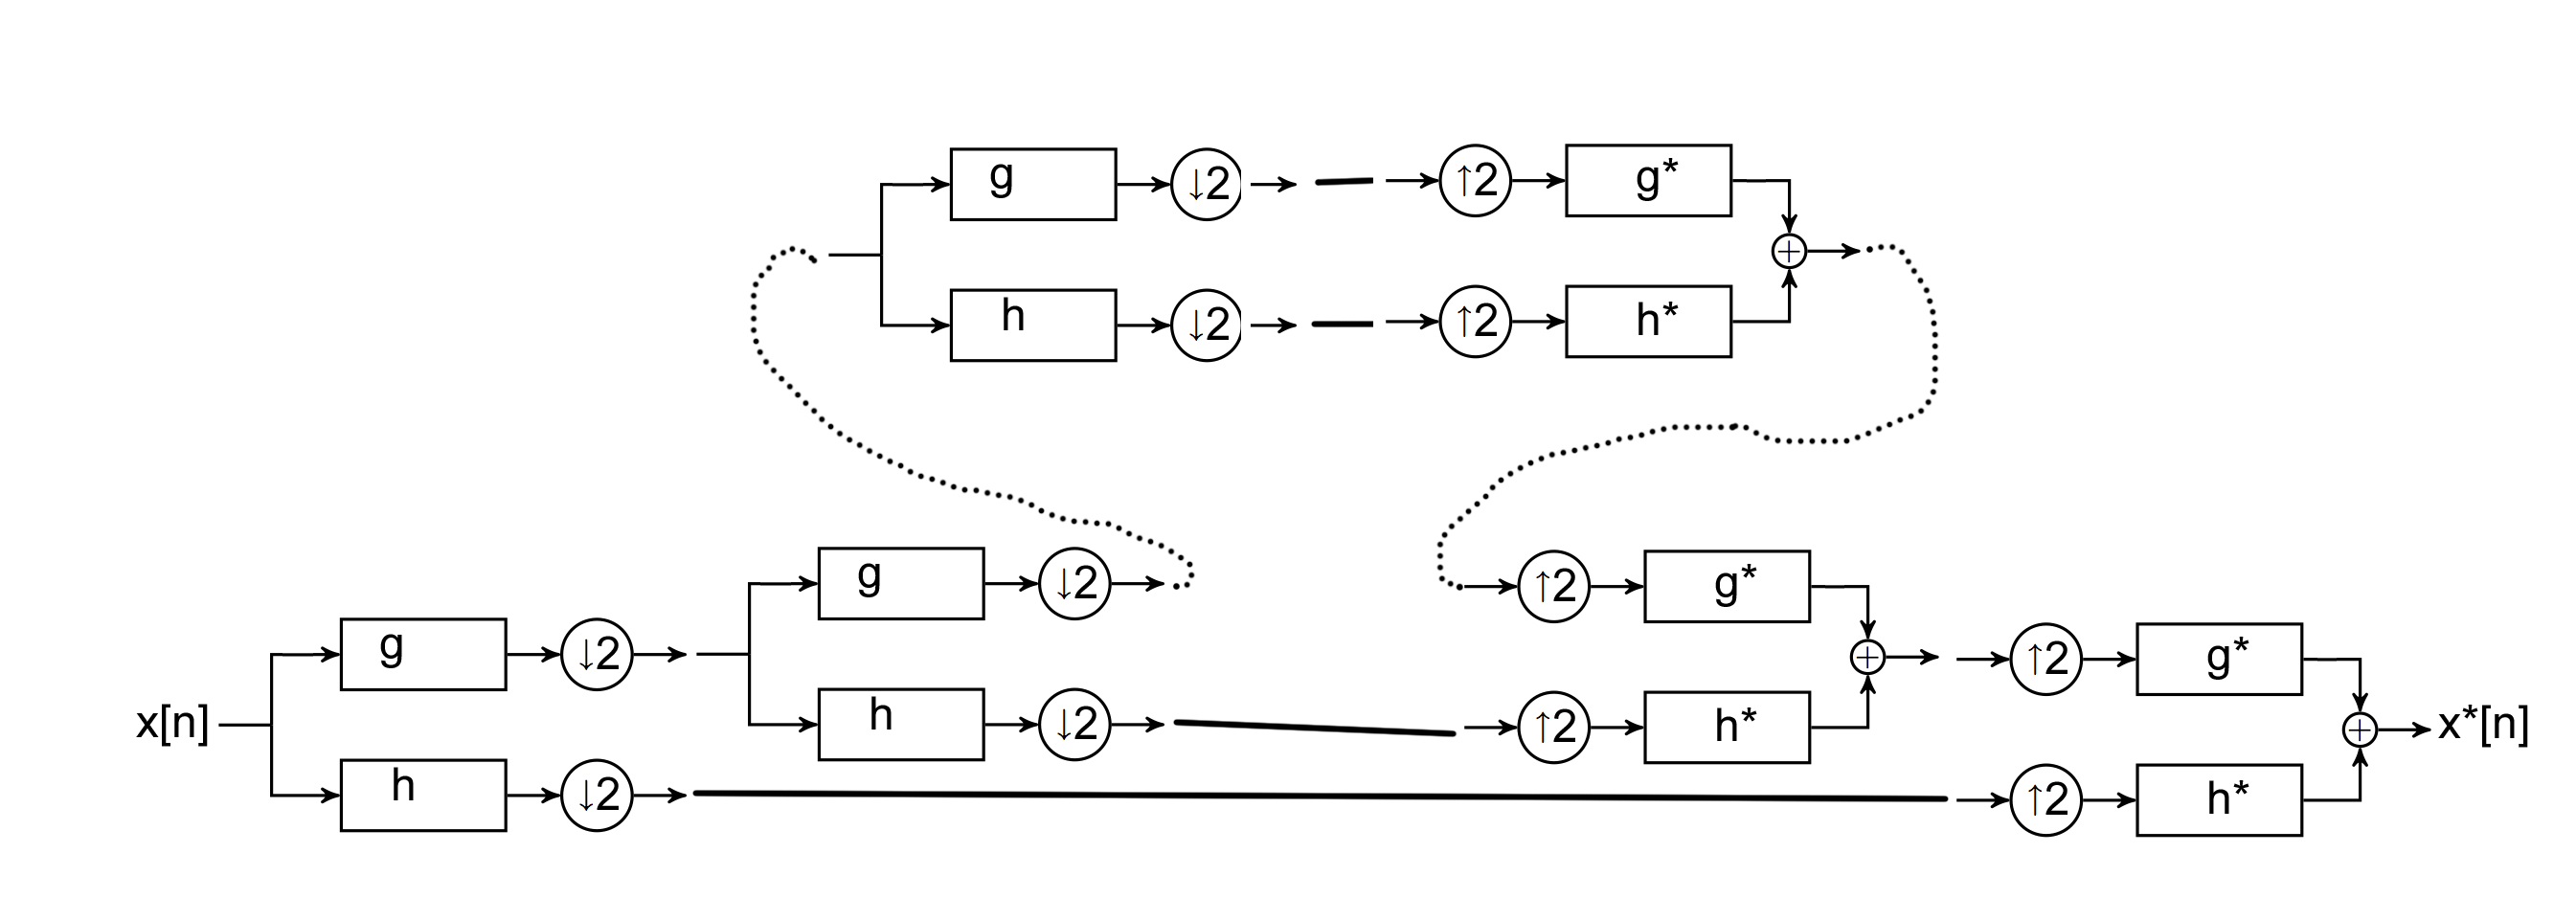
\includegraphics{filter_bank_kankerzuur.jpg}
\end{figure}

Hiermee wordt ook direct het inverse algoritme duidelijk. Gegeven een verzameling rijen $\{y_h, y_{lh}, y_{llh}, \ldots, y_{l^nh}, y_{l^nl}\}$ kunnen we in elke stap het originele signaal $x[n]$ terugvinden door, gegeven de $y_l, y_h$ van die stap:
\[
	y^*_{l}[n] = \begin{cases} y_{l}[n/2] &\text{als } n \mod{2} \equiv 0 \\ 0 &\text{anders}; \end{cases}
\]
\[
	y^*_{h}[n] = \begin{cases} y_{h}[n/2] &\text{ als } n \mod{2} \equiv 0 \\ 0 &\text{anders}. \end{cases}
\]
\[
	x[n] = \sum_{k=-\infty}^\infty y^*_{l}[k]g^*[n-k] + \sum_{k=-\infty}^\infty y^*_{h}[k]h^*[n-k].
\]
Herhaald toepassen van dit geeft het originele signaal terug\footnote{Mits er onderweg geen verlies van preciesie plaats heeft gevonden.}.
\end{algoritme}

Een klein voorbeeld. De meest simpele Wavelet is de Haarwavelet, uitgevonden door Alfred Haar in 1909. De term Wavelet werd echter pas veel later genoemd.

De Haarwavelet is als volgt gedefinieerd:
\[
	\psi(x) = \begin{cases} 1 & \text{als } x \in [0,\frac{1}{2}] \\ -1 & \text{als } x \in [\frac{1}{2},1] \\ 0 & \text{anders.} \end{cases}
\]
\[
	\phi(x) = \begin{cases} 1 & \text{als } x \in [0,1] \\ 0 & \text{anders.} \end{cases}
\]
De filters die we hierbij vinden worden dus
\[
	h[n] = (-\frac{1}{2}\sqrt{2},\frac{1}{2}\sqrt{2}); g[n] = (\frac{1}{2}\sqrt{2},\frac{1}{2}\sqrt{2}); h^*[n] = (\frac{1}{2}\sqrt{2},-\frac{1}{2}\sqrt{2}); g[n] = (\frac{1}{2}\sqrt{2},\frac{1}{2}\sqrt{2}).
\]

Stel we hebben een signaal $(1,2,1,2,3,4,3,4)$. Dan vinden we met de eerste stap
\[
	y_l = \frac{1}{2}\sqrt{2}\cdot(3,3,7,7); y_h = \frac{1}{2}\sqrt{2}\cdot(-1,-1,-1,-1)
\]
en daarna
\[
	y_{ll} = (3, 7); y_{lh} = (0, 0)
\]
en daarna
\[
	y_{lll} = \frac{1}{2}\sqrt{2}(10); y_{llh} = \frac{1}{2}\sqrt{2}(-4).
\]

Ons uiteindelijke getransformeerde signaal wordt
\[
	y = (y_{lll},y_{llh},y_{lh},y_{h}) = \frac{1}{2}\sqrt{2}(10, -4, 0, 0, -1, -1, -1, -1).
\]

\section{Compressie}
Wanneer we nu deze verzameling $\{y_h, y_{lh}, y_{llh}, \ldots, y_{l^nh}, y_{l^nl}\}$ `aan elkaar plakken' tot een rij $y[n]$ met dezelfde lengte als het oorspronkelijke signaal kunnen we op dezelfde wijze als bij de Fouriertransformatie co\"effici\"enten die kleiner zijn dan een bepaalde waarde $\e$ weggooien. Dit kan natuurlijk op twee manieren: 
\begin{itemize}
\item Laat $\e$ vast en bepaal daarmee hoeveel er weggegooid wordt;
\item Laat het compressieniveau\footnote{de fractie nog overgebleven co\"effici\"enten} $p \in (0,1]$ vast en bepaal een $\e_p$ aan de hand hiervan.
\end{itemize}

Wij hebben in onze implementatie gekozen voor de tweede optie

\section{In meer dimensies}

\subsection{Mallat versus Tensor}
Plaatje

\section{Results}
Terminology: PSNR, implementatie (snippets)

\subsection{pt 1: plaatjes}
\subsection{pt 2: filmpjes}

-----

\section{discussion}

BRONNEN
\fi

\end{document}
